\documentclass[a4paper,11pt]{kth-mag}
\usepackage[T1]{fontenc}
\usepackage{textcomp}
\usepackage{lmodern}
\usepackage[utf8]{inputenc}
%\usepackage[latin1]{inputenc}
\usepackage[swedish,english]{babel}
\usepackage{modifications}
\title{A comparison of sudoku solving algorithms}

\subtitle{by ability in solving, generation and difficulty rating of sudoku puzzles.}
\foreigntitle{En jämförelse av algoritmer för lösning av sudokupussel}
\author{Patrik Berggren \and David Nilsson}
\date{April 2012}
\blurb{Bachelor's Thesis at NADA\\Supervisor: Alexander Baltatzis\\Examiner: Mårten Björkman}
\trita{TRITA xxx yyyy-nn}
\begin{document}
\frontmatter
\pagestyle{empty}
\removepagenumbers
\maketitle
\selectlanguage{english}
\begin{abstract}
This is a bachelor thesis that studies and compare four different sudoku
solving algorithms. Those algorithms are rulebased, backtracking, neural network and 
cultural genetic.  The comparison consisted of measuring the algorithms, including
variations of the algorithms, against a database of 49 151 different 17-clue sudoku
puzzles. The algorithms use in generating as well as rating difficulty in sudoku
puzzles was also compared. The results show that ...
\end{abstract}
\clearpage
\begin{foreignabstract}{swedish}
TODO: Översätt abstract från engelska när den är färdig så att det är samma sak som står.
\end{foreignabstract}
\clearpage
\tableofcontents*
\mainmatter
\pagestyle{newchap}
\chapter{Introduction}
Sudoku is a game that under recent years have gained popularity throughout the world. 
The game consists of a 9 by 9 grid which shall be filled in so that each 
row, column and 3 by 3 square (also called a box) contains the digits 
1 through 9 exactly ones. 
Many newspaper today contain sudoku puzzles and there are also competitions devoted 
to sudoku solving. It is therefore of interest to study how one can generate, 
solve and rate such puzzles by the help of computers.

\section{Problem specification}
To generate and solve sudokus one can choose from several different algorithms. 
Some might be limited to only generation or only solving whilst other could be used for both. 
The main goal of this project is to explore different aspects of sudoku solving and generation.
To be able to compare different ideas, several algorithms will be used in the comparison. 
The project will not only try to identify which algorithm seems to fit best for 
a specific aspect of sudoku, but also conclude how each algorithm performs itself and why.
\newline
The algorithms that will be studied are backtrack solver, ruledbased solver, 
nueral network solver and cultural genetic solver. 
Those will be discussed and explained in more detail in section 2.1 and 3. 
Variations of those algorithms will also be studied so there will in effect 
be data for 10 or more algorithms and variations of algorithms.
\newline
The ideas that will be studied are how well each algorithm performs on a given set of puzzle. 
The algorithms will be compared towards each other and hopefully it will be possible to make 
conclusions about which kind of algorithm effectively solve which kind of puzzles. 
Each sudoku solving algorithm can also be used for sudoku generation, which is another 
aspect that will be studied and compared in this project. Furthermore some implementation 
issues regarding the algorithms will be discussed, 
such as how well the algorithms are suited for parallelising the work. 
The discussion will also touch on difficulty rating which is another aspect that often 
gets attention in many studies regarding sudoku.

\section{Scope}
As this project is quite limited in time available and in expected scope, 
there are several limitations on what can and will be done. 
These are the limitations of the project:
\begin{itemize}
    \item Limited number of algorithms: Since many of the algorithms are only available as psuedo-code and since we ourselves want to make sure that the algorithms we implement have a similar amount of optimization, we will implement the algorithms ourselves. This will however be time consuming and since each algorithm have multiple variations, the measurements will also be time consuming. The analysis would also be beyond this scope if to many algorithms were chosen.
    \item Optimization: As mentioned above we will put some work into optimizing the different algorithms, but it will however be limited to which extent this can be done. This will affect the conclusion as some comparisons might have some uncertianty regarding the correctness of the results. The general idea is to put the same amount of work into every algorithm, while keeping the essential parts of the program in mind.
    \item Special sudokus: There are several variations of sudoku including different sizes of the grid. This thesis will however be limited to the study of ordinary sudoku, which is 9 by 9 grids.
    \item The results of this thesis will be applicable to other areas apart from sudoku related topics, but those will only be mentioned briefly and no extensive study regarding the use of the results in other areas will be done. 
\end{itemize}

\section{Purpose}
As already mentioned, sudoku is today a popular game throughout the world and it appears 
in multiple medias, including websites, newspapers and books. 
As a result, the demand of effective sudoku related algorithms are rising. 
For most purposes there already exist satisfactory algorithms, but there are 
still some value in studying sudoku algorithms. 
Sudoku could for instance be extended to a more generalized form with 
a n by n grid and most regular sudoku solving algorithms could be generalized 
to solve those as well. 
Another related reason for studying sudoku solving algorithms is that there exists 
several similar problems to sudoku and an idea for sudoku may be applicable for 
those other related puzzles. 
Latin squares are for instance a very similar puzzle that could directly benefit 
from sudoku solving algorithms. 
There are however a broader class of problems that could benefit from these thesis 
and those are the NP-complete problems. 
Sudoku is one of those NP-complete problems \cite{complexity} which briefly speaking means that 
no known effective algorithm exists that solve them. 
For now we will however only conclude that there exists some similarities between 
sudoku and some of those NP-complete problems, such as latin squares and graph colouring. 

\section{Background}
Ever since sudoku started to get popular in the 80s it have been studied from different perspectives by both computer scientists and mathematicans. Many of those results have some impact on this thesis since many different aspects are studied. Some results that are of value but of minor direct use is the proof for sudokus NP-completeness \cite{complexity} and the proof that the minimal number of clues in a puzzle is 17. \cite{17clueProof} Enumeration of sudoku solutions is also relevant to this thesis in order to give a clearer picture of how big the search space is for solutions. \cite{enumeration} 

The most important sources are the ones that concern the algorithms. Primarly the chosen algorithms, but some other reports concerning other algorithms may also be of interest. Those directly related to the chosen algorithms are. \cite{techniques,boltzmann,stochastic,review} There are however as mentioned also some other articles that have helped in both chosing of the algorithms, but also by algorithmic ideas that can be used. Those articles and webpages are. \cite{discrepancySearch,culturalSwarms,culturalSwarms}

As mentioned in the problem specification this thesis will not only be concerned with solving sudoku puzzles but also generating them and \cite{generation} have been of great help by discussing this topic from different aspects which mainly includes how one shall generate puzzles using different sudoku solving algorithms in reverse.

One of the most important resources to this project is the puzzles used in the comparisons and those were collected from. \cite{database} There also exists some tools which was used in the analysis and those were. \cite{13,14,15,16}


%%\part{Important Results}

\chapter{Method}
Since this report have several aims, this section have been divided into different parts to clearly depict what aspects have been considered regarding the different aims. Section 2.1 is devoted to explaining how and which algorithms was chosen and section 2.2 explains which puzzles are used as benchmarks and why. Section 2.3 explains how the comparison was carried out regarding the different aspects that was studied.

\section{Chosen algorithms}
There are as already mentioned in the introduction several algorithms for solving sudoku. It would be of interest to do a quantative study of those to definitely determine which ones that performs best. Due to limitations of this study and to make the study of the chosen algorithms more qualitativly, four algorithms have been chosen. The main selection criteria was that they offered a new approach in relation to the other algorithms. The algorithms that was chosen are the following:
\begin{itemize}
    \item Backtracking: Backtracking is probably the most basic sudokusolving strategy for computer algorithms. It is a kind of a bruteforce method which tries different numbers and if it fails it backtracks and try a different number.
    \item Ruledbased: This method consists of using several rules that logically proves that a square either must have a certain number or roles out numbers that are impossible (which for instance could lead to a square with only one possible number). This method is very similar to how humans solve sudoku and the rules used is in fact derived from human solving methods.
    \item Cultural genetic: 
    \item Nueral Network: Modelling a sudoku by using a constraint solving artificial neural network. The most natural way of encoding constraints is with a reccurent stochastic boltzmann network. By overlaying the input grid over all neural network nodes and then simulating until it is stable, a valid solution can be found. This way of solving constraint problems can be seen as a natural way of encoding data and constraints. It is however difficult to reason about performance.
\end{itemize}

As the reader probably notices, this algorithms are quite different from each other. Both in which ideas are used but also in which algorithm constructing methods. Our hopes for this project is therefore that we will be able to determine how those algorithms could be used in several situations for either generating or solving sudokus. The implementations of those algorithms will be discussed in more detail in section 3. 

\section{Benchmark puzzles}
This thesis relies highly on measuring how long it takes different algorithms to solve puzzles. To measure this, puzzles are needed and consideration shall therefore be taken to choose those puzzles wisely. The puzzles that have been chosen to test the solving capabilities of the algorithms are a collection consisting of 49 151 puzzles which each have 17 clues (meaning 17 squares are filled in). \cite{database} Those have been collected by Gordon Royle from different sites as well as from his own database. The reason for choosing this collection is because it is believed not to be biased towards a specific solving idea. This is because it is a collection that comes from collecting as many of the 17-clue puzzles that have been found as possible rather than using a specific generation method. The collection also have other benefits. The puzzles are all qualitativly different as no pair of puzzles is within the same equivalence class. Equivalent puzzles are defined as puzzles that could be transformed into each other using some predefined operations that doesnt change the solution. One might for instance interchange the digits in a puzzle, but the solution would then be the transformed solution and no real change to the puzzle have therefore been done. Some other operations includes interchanging rows, columns and stacks (three boxes in a row,column). The downside of choosing this collection is that some algorithms may perform poorly because of the low nr of clues given and some analysis of this will therefore be carried out. This will be done by solving the given puzzles and adding some of the numbers in the solution to the puzzle. The reason for this approach is ones again that one does not want to rely too much on a specific generation method.

\section{Comparison methods}
As already mentioned several comparisons and measurements will be carried out to 
analyse different aspects of the algorithms. Those will include statistically tests 
to for instance determine with what confidence one can say that one algorithm performs 
better than another. 
The following subsections will however explain more clearly what will be measured 
regarding each aspect. 
Two of the general problems one most confront when doing this kind of study is how one 
shall make sure that the measured time for  running a algorithm is correct. 
There might for instance be delays due to slow input and output and one must also account 
to variations in runningtime. 
The input/output delays can be avoided by communicating with the algorithm through a 
direct interface. 
Variations in runningtime is however difficult to predict, but one might however use a 
meanvalue as a approximation. 
To some extent the variations of the runningtimes will be reduced as the algorithms are tested against a large set of puzzles.  

\subsection{Solving}
The main interest of this thesis is the algorithms ability to solve sudokus and most focus will therefore also be on measuring their solving abilities. As already mentioned, there is a fixed collection of puzzles that shall be tested on each algorithm and also on each variation of the algorithms. The data needed for the analysis will consist of measuring the time it takes for each algorithm to solve each puzzle. This will result in quite a big data set and consideration must therefore be taken regarding what statisticall methods are used to analyse it. 
\underline{(It is however at this point not decided which stasticall tests shall be performed so a discussion of that is yet to come).}

\subsection{Generation}
Sudoku solving algorithms may also be used to generate puzzles. One way this could be done in is by randomly placing numbers in squars and then using the solver to determine if there is a sudoku and if it is unique. Some solvers may however be better suited for this as some will for example not be vary suited for determining if a solution is unique. There are however also other methods for generating puzzles as explained in \cite{generation}. The algorithms will therefore be compared at theirs ability to generate puzzles in any way that the authors thinks suitable. The comparison will regard how correct the generated puzzles are (if there is always a unique solution) and also how fast the generation was done. As the data from the generation testing will be very similar to the data from the solving tests, the same statistical tests will be used.

\subsection{Parallelising}

\subsection{Difficulty rating}

\section{Implementation}

In this section we will describe the methods in more detail and also explain which modifications that might be interesting to do to each algorithm. Parallelising the algorithms will also be discussed alldue the comparison of this will still be in section 4.

\subsection{Backtracking}

The backtracking algorithm for solving sudoku is a bruteforce method. One might view it as guessing which numbers goes where. When a deadend is reached, the algorithm backtracks to a earlier guess and tries something else. This means that the backtracking algorithm does an extensive search to find a solution. The main drawback to this algorithm is that it is exponential in time complexity, but will on the other hand always find a solution sooner or later if one exists. This method may also be used to determine if a solution is unique for a puzzle as the algorithm can easily be modified to continue searching after finding one solution. As a result it could be used to generate valid sudoku puzzles (with unique solutions).
\newline
Parallelising is something that could improve this algorithm considerable. The way this could be done is by searching different searchpaths in parallel. This is possible as the search three is fixed and only determined by the puzzle.
\newline
There are several interesting variations of this algorithm that might prove to vary in effiecency. The main variations regards in which order the squares are visited. One might for instance search the squares in random order or in some order that is defined by the structure of the sudoku. One might for instance first fill in all possible numbers in each empty square and then begin with the least number of candidates, or one might want to finish nearly completed rows, columns or boxes. One might also vary how the guesses are done. Some rules regarding how the guesses are done might lead to a higher probability to find a solution which in turn will make the whole algorithm faster as the solutions will be found earlier in the search.

\subsection{Ruledbased}
This algorithm relies on the logic rules that humans use to solve sudoku. Those rules works as proofs and either determines that a square must be a certain number or prooves that a certain square can not contain a certain number. The rules that are used are as follows:
\begin{description}
    \item[Naked Single] 
    This means that a square only have one candidate number.
    \item[Hidden Single] 
    If a row, column or box contains only one square which can hold a specific number then that number must go into that square.
    \item[Naked pair] 
    If a row, column or box contains two squares which each only have two specific candidates. If one such pair exists, then all occurences of these two candidates may be removed from all squares that share a row, column or box with both of the squares in the pair. This concept can also be extended to three or more squares.
    \item[Hidden pair]
    If a row, column or box contains only two squares which can hold two specific candidates, then those squares are a hidden pair. It is hidden because those squares might also include several other candidates. Since one already know which two numbers have to go into the two squares one might remove other candidates for those two squares. Those squares will now be a naked pair and one could therefore apply the rule for removal of further candidates. Similar to naked pairs this concept may also be extended to three or more squares.

    \item[X-wing/swordfish/jellyfish/squirmbag]
    These are all names of a more general rule that concerns a loop. Below is a example of a so called swordfish (figure 1 and 2). In figure 1 the squares which have the digit 4 as a candidate have been marked. The so called swordfish is shown in figure 2. The logical reasoning one might use with a swordfish is that since the configurations of the fours in the swordfish can only take two configurations and both of them will cover the same set of columns and rows. The other squares in those rows and columns with the digit 4 as a candidate may therefore remove 4 as a candidate. Swordfish is the special case of this concept where 3 rows and columns are involved in the loop, but the concept also applies to loops within 2 rows and columns (X-wing) and even loops with more than 3 rows and columns involved (jellyfish and squirmbag).

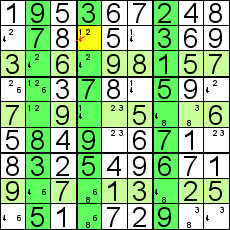
\includegraphics{images/swordfish1.png}
\newline
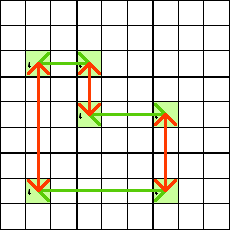
\includegraphics{images/swordfish2.png}

\end{description}

There are other rules that could be used but due to limitations these are the only implemented ones. There are several different aspects that are interesting to note about this algorithm. First of all the time complexity of the algorithm will be polynomial given that a solution can be found using these rules. This is a simple consequence of the fact that each rule only take polynomial time to check and there are only polynomial many squares to fill in. There are however no guarantee that a solution will be found and if no rule match it is impossible for the algorithm to continue. One way around this is to combine this algorithm with the backtracking algorithm. Other aspects that shall be studied are which rules shall be applied in which order and even if some rules are to time consuming to check compared to the extra puzzles that can be solved. The variations of this algorithm therefore consists of different sets of rules (including guessing rules for backtracking) that are applied in different orders. 

\subsection{Cultural genetic}

A cultural genetic algorithm is a basic genetic algorithm with additional inputs determining properties of the search for a solution.
 There are some basic components that are common to all genetic appropaches. \newline
When dealing with a problem space with many possible solutions it is common to define a population which consists of individuals.
Every individual represents a single possible sudoku puzzle solution.
Every individual has a single integer for every not given square, that represent the yet to be filled sudoku grid, and therefore every integer is limited to the range between one and nine.
All these integers are known as genes and describes the solution proposed by a certain individual. \newline
Given the search space representation there is also a method of successively building up better individuals and a population that, overall, achieves better sudoku solutions.
In order to determine how good any individual is in relation to another a fitness function is defined.
This is simply the number of reused or missing integers, giving a good measure of the quality of a proposed solution.
During simulation the fitness function is evaluated for every individual.
The best individuals are then chosen for a tournament process.
This will reduce the number of candidates available for coming populations, and determine which individuals that are combined.
Finally a few individuals are combined in a process known as crossover.
This simply selects genes from both candidates and constructs a new individual.
After constructing the final candidate there might also be mutations in the genes, allowing the search to avoid a local minima.
The process is repeated until a proper puzzle candidate has been found.
The reader might note that a correct solution will have minimize the fitness function. \newline
The cultural part of ``cultural genetic`` implies that the environment in some way controls how the search goes on.
The cultural effects are labeled belief space and makes sure that gene selection only takes valid values and that repetition is avoided.
This can be seen as a way of introducting constraints.

\subsection{Artificial neural network}
In order to fully understand the artifical neural network approach of solving sudoku puzzles, it is necessary to have some basic theoretical background before introducting the implementation.

\subsubsection{Artificial neural network - theory}
The artificial neural network solver is based on reccurrent stochastic networks that encode all properties of sudoku. In the core there is a Boltzmann machine, which can be seen as a network of fully connected nodes, as pictured below.

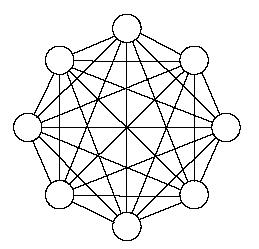
\includegraphics{images/neural1.png}

The recurrent property implies that output connections are fed back into to neurons, or in this case, all nodes are fully connected.
This definition often implies a hopfield network which is a somewhat limited version of the Boltzmann machine.
What differentiates them and makes the latter more powerfull is the stochatic property, meaning state transitions of individual nodes are stochastic.

In the case of sudoku there are a total of 81*9 nodes; for every number being placed on the grid, there is nine possible assignments.
When a solution is present in the network there will only be one node active in every group and the solution can be extracted by simply assigning the node index within the group as the resulting grid number.

Given that a network of nodes has been defined it is also required to encode constraints.
This is done by introducing weights on all edges in the fully connected network.
All weights are stored in a weight matrix that satisfies the following conditions:

\[
w_{ii} = 0 \quad \forall i
\]
\[
w_{ij} = w_{ji} \quad \forall i,j
\]

At any moment in the simulation there is a state present in the network, which is coded separately.
Each node has a binary state s\_i of either on or off.
This also translates to solutions, where only one of every nine neurons in groups will be in the state on.
With weights and the state associated with every node of the network it is also useful to define an energy measure which is used to determine if the state of single neuron should be flipped.
The difference in enery activation for a single node flipping state is given by the following equation, where theta is a offset used as an adjustable performance parameter \cite{boltzmann2}:
\[
\Delta E_{i} = \sum_{j} w_{ij} s_{j} - \theta
\]

Due to stochastic nature of boltzmann machines there is a separate probability function used to determine if a single neuron should flip its state during a discrete time step \cite{boltzmann2}.
Here another adjustable performance parameter is introduced, T.
In order to have convergence in the network towards a valid sudoku solution it is necessary to control the probablity of state flipping as the simulation goes on.
This is done by utilising simulated annealing which controls the temperature T over time.
By lowering the value in a controlled fashion it is possible to maximize the probability of a final correct solution.
\[
p_{i=on} = \frac{1}{1+e^{-\frac{\Delta E_{i}}{T}}}
\]

\subsection{Artificial neural network - implementation}

Using the previously introduced expressions it is now possible to describe the actual implemenation and the steps necessary to solve sudoku puzzles.
\newline

The first step is to take initialize a random weight matrix and random states for all 81*9 nodes in the neural network.
Then all given grid values are inserted as activiations of states in the associated groups of neurons, with all others being set to the off state.
This ensures that only the given activations are active.
\newline

The second step is to encode sudoku restrictions into the weight matrix.
Negative connections are introduced between different digits on within the same group, in other words only one digit should be active on every place in the grid at the same time.
The other properties of unique rows, unique columns and unique subsquares are encoded in the same way but processed with the whole weight matrix.
\newline

With all configuration done it is then time to launch the simulation, which is run in discrete time steps.
At every time step the energy function is evaluated at all nodes.
The energies are then processed which renders the probablities of nodes flipping state, which is then performed to varying degrees.
Since simulated annealing is used with a lowered temperature T there also small adjustments at certain intervals.
This is done in a timely manner which allows all puzzles to be solved but still doesn't waste any time for uneccessary computation.
\newline
A valid solution can be found by simple looking at all states and insepecting the requirements of sudoku.
Commonly the solution will appear in the end of the simulation when temperaure has been lowered to its minimum.
\section{Comparison}

At this point, the conclusions that can be drawn are very limited. This is largerly due to the fact that the test system have not yet been implemented even thought the first draft of the algorithms have been implemented. Some tests so far however show that the ruledbased solver seems to be able to solve roughly 50\% of the puzzles with only hidden and naked single rules. Since puzzles that only requires these rules are generally regarded as very easy puzzles, one can conclude that most sudoku puzzles probably are easy. An hypothesis that is related to that but not yet tested is that it will probably be difficult to generate difficult problems. Backtracking algorithms with some variations have also been tested, but at a smaller scale. It seems so far that backtracking seems to be a less fit algorithm for solving 17-clue puzzles, but some optimization are yet to be done. 
Those are the subsections expected to exist in the finished report.
\subsection{Solving}

This will probably be the most extensive subsection and it will probably be divided into smaller parts. It is however difficult to tell which those will be now since they greatly depend on what results we get.
\section{Generation}

\section{Parallelising}

\section{Difficulty ratings}


\section{Conclusion}

There is as mentioned in comparison not much to conclude at this point since the real comparison have not yet been carried out.


\section{References}

\begin{thebibliography}{99}

\bibitem{complexity}
Takayuki Y, Takahiro S. Complexity and Completeness of Finding Another Solution and Its Application to Puzzles. [homepage on the Internet]. No date [cited 2012 Mar 8]. Available from: The University of Tokyo, Web site: http://www-imai.is.s.u-tokyo.ac.jp/~yato/data2/SIGAL87-2.pdf

\bibitem{17clueProof}
Tugemann B, Civario G. There is no 16-Clue Sudoku: Solving the Sudoku Minimum Number of Clues Problem. [homepage on the Internet]. 2012 [cited 2012 Mar 8]. Available from: University College Dublin, Web site: http://www.math.ie/McGuire\_V1.pdf

\bibitem{enumeration}
Felgenhauer B, Jarvis F. Enumerating possible Sudoku grids. [homepage on the Internet]. 2005 [cited 2012 Mar 8]. Available from: University of Sheffield, Web site: http://www.afjarvis.staff.shef.ac.uk/sudoku/sudoku.pdf

\bibitem{techniques}
Astraware Limited. Techniques For Solving Sudoku. [homepage on the Internet]. 2008 [cited 2012 Mar 8]. Available from:, Web site: http://www.sudokuoftheday.com/pages/techniques-overview.php

\bibitem{boltzmann}
Ekeberg. Boltzmann Machines. [homepage on the Internet]. 2012 [cited 2012 Mar 8]. Available from:, Web site: http://www.csc.kth.se/utbildning/kth/kurser/DD2432/ann12/forelasningsanteckningar/07-boltzmann.pdf

\bibitem{stochastic}
Marwala T. Stochastic Optimization Approaches for Solving Sudoku. [homepage on the Internet]. 2008 [cited 2012 Mar 8]. Available from:, Web site: http://arxiv.org/abs/0805.0697

\bibitem{review}
. An Incomplete Review of Sudoku Solver Implementations. [homepage on the Internet]. 2011 [cited 2012 Mar 8]. Available from:, Web site: http://attractivechaos.wordpress.com/2011/06/19/an-incomplete-review-of-sudoku-solver-implementations/

\bibitem{discrepancySearch}
Harvey W, Ginsberg M. Limited discrepancy search. [homepage on the Internet]. No date [cited 2012 Mar 13]. Available from: University of Oregon, Web site: http://citeseerx.ist.psu.edu/viewdoc/download?doi=10.1.1.34.2426\&rep=rep1\&type=pdf

\bibitem{searchBased}
Cazenave Cazenave T. A search based Sudoku solver. [homepage on the Internet]. No date [cited 2012 Mar 13]. Available from: Université Paris, Dept. Informatique Web site: http://citeseerx.ist.psu.edu/viewdoc/download?doi=10.1.1.64.459\&rep=rep1\&type=pdf

\bibitem{culturalSwarms}
Mantere T, Koljonen J. Sudoku Solving with Cultural Swarms. AI and Machine Consciousness [homepage on the Internet]. 2008 [cited 2012 Mar 13]. Available from: University of Vaasa, Department of Electrical Engineering and Automation Web site: http://www.stes.fi/step2008/proceedings/step2008proceedings.pdf\#page=60

\bibitem{generation}
Morrow J. Generating Sudoku Puzzles as an Inverse Problem. [homepage on the Internet]. 2008 [cited 2012 Mar 13]. Available from: University of Washington, Department of Mathematics Web site: http://www.math.washington.edu/~morrow/mcm/team2306.pdf

\bibitem{database}
Royle G. Minimum Sudoku. [homepage on the Internet]. No date [cited 2012 Mar 13]. Available from: The University of Western Australia, Web site: http://www.math.washington.edu/~morrow/mcm/team2306.pdf

\bibitem{boltzmann2}
Ackley D, Hinton G. A Learning Algorithm for Boltzmann Machines. [homepage on the Internet]. 1985 [cited 2012 Mar 13]. Available from: The University of Western Australia, Web site: http://learning.cs.toronto.edu/~hinton/absps/cogscibm.pdf

\end{thebibliography}

\appendix
\addappheadtotoc
\chapter{RDF}\label{appA}

\begin{figure}[ht]
\begin{center}
And here is a figure
\caption{\small{Several statements describing the same resource.}}\label{RDF_4}
\end{center}
\end{figure}

that we refer to here: \ref{RDF_4}
\end{document}
